%%%%%%%%%%%%%%%%%%%%%%%%%%%%%%%%%%%%%%%%%
% Dreuw & Deselaer's Poster
% LaTeX Template
% Version 1.0 (11/04/13)
%
% Created by:
% Philippe Dreuw and Thomas Deselaers
% http://www-i6.informatik.rwth-aachen.de/~dreuw/latexbeamerposter.php
%
% This template has been downloaded from:
% http://www.LaTeXTemplates.com
%
% License:
% CC BY-NC-SA 3.0 (http://creativecommons.org/licenses/by-nc-sa/3.0/)
%
%%%%%%%%%%%%%%%%%%%%%%%%%%%%%%%%%%%%%%%%%

%----------------------------------------------------------------------------------------
%	PACKAGES AND OTHER DOCUMENT CONFIGURATIONS
%----------------------------------------------------------------------------------------

\documentclass[final,hyperref={pdfpagelabels=false},noamsthm]{beamer}

\usepackage[orientation=portrait,size=a0,scale=1.4]{beamerposter} % Use the beamerposter package for laying out the poster with a portrait orientation and an a0 paper size

\usetheme{I6pd2} % Use the I6pd2 theme supplied with this template

\usepackage[english]{babel} % English language/hyphenation

\usepackage{amsmath,amsthm,amssymb,latexsym} % For including math equations, theorems, symbols, etc

\usepackage[document]{ragged2e}
\usepackage{multicol}

\usepackage{algorithmicx}
\usepackage{algorithm}
\usepackage{algpseudocode}

\newtheorem{proposition}{Proposition}

\usepackage{tikz}
\usetikzlibrary{fit}					% fitting shapes to coordinates
\usetikzlibrary{backgrounds}	% drawing the background after the foreground

%\usepackage{times}\usefonttheme{professionalfonts}  % Uncomment to use Times as the main font
\usefonttheme[onlymath]{serif} % Uncomment to use a Serif font within math environments

%\boldmath % Use bold for everything within the math environment

\usepackage{booktabs} % Top and bottom rules for tables

\graphicspath{{figures/}} % Location of the graphics files

\usecaptiontemplate{\small\structure{\insertcaptionname~\insertcaptionnumber:} \insertcaption} % A fix for figure numbering

\usetikzlibrary{arrows}

\newcommand{\shrink}{-15pt}
\newcommand{\shrinkend}{-12pt}

\def\imagetop#1{\vtop{\null\hbox{#1}}}

\newcommand{\norm}[1]{\left\lVert#1\right\rVert}
\newcommand{\E}{\mathbb{E}}
\DeclareMathOperator{\MSE}{MSE}
\newcommand{\asto}{\overset{a.s.}{\to}}

\theoremstyle{plain}
\newtheorem{theorem}{Theorem}

\theoremstyle{remark}
\newtheorem{remark}{Remark}

\theoremstyle{lemma}
\newtheorem{lemma}{Lemma}

\newcommand{\hg}{\hat{\gamma}}
\newcommand{\gy}{\gamma(y)}
\newcommand{\gyn}{\gamma(y_n)}
\newcommand{\real}{\mathbb{R}}

\DeclareMathOperator*{\argmax}{arg\,\!max}


\newenvironment<>{mytheorem}[1][]
{\alert{\upshape\textbf{Theorem}} #1\hspace*{\fill} \\
	\itshape}
{}
\makeatletter
\newenvironment<>{myproof}[1][\proofname]{%
	\par
	\def\insertproofname{#1\@addpunct{.}}%
	\pushQED{\qed}
	\alert{\textbf{\insertproofname}} \hspace*{\fill} \\}
{\popQED}
\makeatother
\usepackage{array}
\newcolumntype{C}[1]{>{\centering\let\newline\\\arraybackslash\hspace{0pt}}m{#1}}

\usepackage{listings}
\usepackage{color}
\usepackage{xcolor}
\usepackage{textcomp}
\usepackage{xspace}

% blackboard series
\def\bbP{\mathbb{P}}
\def\bbp{\mathbb{p}}
\def\bbE{\mathbb{E}}
\def\bbN{\mathbb{N}}

% calligraphic series
\def\calT{\mathcal{T}}
\def\calW{\mathcal{W}}
\def\calX{\mathcal{X}}

% bold series
\def\bfP{\mathbf{P}}
\def\bfX{\mathbf{X}}

% distributions
\def\aDist{\Lambda}
\def\aTime{T}
\def\Geom{\text{Geom}}

% stuff
\newcommand{\prob}{\mathbb{P}}
\newcommand{\calV}{\mathcal{V}}
\newcommand{\calE}{\mathcal{E}}
\newcommand{\ee}{Z} % ends of edges
\newcommand{\bfee}{\mathbf{\ee}}
\newcommand{\bfE}{\mathbf{E}}
\newcommand{\PYP}{\mathcal{PYP}}
\newcommand{\geom}{\beta}
\newcommand{\BNTL}{\text{\rm BNTL}}
\newcommand{\bfT}{\mathbf{T}}
\newcommand{\calO}{\mathcal{O}}
\newcommand{\bbR}{\mathbb{R}}
\newcommand{\bfPsi}{\boldsymbol{\Psi}}
\newcommand{\bfn}{\mathbf{n}}
\newcommand{\bfd}{\mathbf{d}}
\newcommand{\argdot}{{\,\vcenter{\hbox{\scalebox{0.5}{$\bullet$}}}\,}}%{\bullet}
\def\indicator{\mathbf{1}}
\newcommand{\limscale}[2]{\overset{\scriptscriptstyle{#1 \uparrow #2}}{\widesim[1.25]}}
\newcommand{\simiid}{\overset{\scriptscriptstyle{\text{i.i.d.}}}{\widesim}}
\newcommand{\widesim}[1][1.5]{
  \mathrel{\scalebox{#1}[1]{$\sim$}}
}


\definecolor{darkgreenClj}{rgb}{0.25,.5,0.25}
\definecolor{blueClj}{rgb}{0,0.33,0.66}
\definecolor{redClj}{rgb}{0.66,0.0,0.0}
\definecolor{purpleClj}{rgb}{0.33,0,0.66}
\definecolor{cyanClj}{rgb}{0.0,0.5,0.5}
\definecolor{orangeClj}{rgb}{0.75,0.35,0.0}
\definecolor{grayClj}{rgb}{0.4,0.4,0.4}
\lstset{ 
	language=Lisp, 
	basicstyle=\small\ttfamily,
	keywordstyle={}, 
	alsoletter={<-,->,:,*,/,?,+,-,/,>,<,=, &},
	commentstyle=\em \color{gray}, 
	frame=lines,
	%float=tbph,
	% captionpos=b,
	showstringspaces=false, 
	keywordstyle=[1]\bf\small\ttfamily\color{blueClj},
	keywords=[1]{BO,theta-best,bo-acquire,sample-initial-points,sample,observe,observe<-,predict,mem,store,retrieve,return,catch,throw,absorb,produce,with-primitive-procedures,conditional,result,log-marginal,mean,collect-results,empirical-mean,
		->sample,->observe,->result},
	keywordstyle=[2]\bf\small\ttfamily\color{redClj},
	keywords=[2]{if,let,letfn,loop,looppredict,recur,or,trampoline,assoc,argmax,count,cons,conj,
		do,first,fn,get,keys,lazy-seq,map,nth,mat/add,mat/div,print,reduce,repeat,repeatedly,rest,set,shape,take,vec,
		when,max,fn?,inc,sample*,observe*},
	keywordstyle=[3]\bf\small\ttfamily\color{cyanClj},
	keywords=[3]{dirichlet-discrete,exponential,flip,gamma,beta,mvn-niw,normal,uniform-continuous,distribution,factor,
		simulate,abc-likelihood,student-t,dirichlet},
	keywordstyle=[4]\bf\small\ttfamily\color{purpleClj},
	keywords=[4]{defopt,defquery,doopt,doquery,query,defdist,infer,checkpoint,exec,defm,cps-of-expression,
		defn,def,declare},
	keywordstyle=[5]\bf\small\ttfamily\color{orangeClj},
	keywords=[5]{:lmh,:ipmcmc,:war,:peace,:log-weight,:result,:id,:dist,:cont,:value,:state,:importance,:smc,:pgibbs,
		:number-of-particles},
	mathescape=true,
	stringstyle={},
	keywordstyle=[6]\bf\small\ttfamily\color{darkgreenClj},
	keywords=[6]{+,-,nil,>,<,*,/,=, &,->>,->},
	mathescape=true,
	stringstyle={},
} 
\lstnewenvironment{code}[2]{\lstset{caption=#1,label=#2}}{}

%\newtheorem{example}{Example} 
%%\newtheorem{theorem}{Theorem}[chapter]
%\newtheorem{lemma}[theorem]{Lemma} 
%%\newtheorem{proposition}[proposition]{Proposition} 
%\newtheorem{remark}{Remark}[chapter]
%%\newtheorem{corollary}[corollary]{Corollary}
%\newtheorem{definition}{Definition}[chapter]
%\newtheorem{conjecture}[conjecture]{Conjecture}
%\newtheorem{axiom}[axiom]{Axiom}

% % % % % % % % % % % % % % % % % % %


%\usepackage{packages/algorithm,packages/algorithmic}
\usepackage{abbreviations}


%----------------------------------------------------------------------------------------
%	TITLE SECTION 
%----------------------------------------------------------------------------------------

\title{\LARGE Sampling and Inference for Beta Neutral-to-the-Left Models of Sparse Networks} % Poster title

\author{\vspace{-5pt} Benjamin Bloem-Reddy, \underline{Adam Foster}, Emile Mathieu, Yee Whye Teh  \vspace{5pt}}
\institute{Department of Statistics, University of Oxford}

%----------------------------------------------------------------------------------------
%	FOOTER TEXT
%----------------------------------------------------------------------------------------

\newcommand{\leftfoot}{} % Left footer text

\newcommand{\rightfoot}{~ \url{http://csml.stats.ox.ac.uk/learning/}} % Right footer text

%----------------------------------------------------------------------------------------


\begin{document}

\addtobeamertemplate{block end}{}{\vspace*{2ex}} % White space under blocks

\begin{frame}[t,containsverbatim] % The whole poster is enclosed in one beamer frame

\begin{columns}[t] % The whole poster consists of two major columns, each of which can be subdivided further with another \begin{columns} block - the [t] argument aligns each column's content to the top

\begin{column}{.02\textwidth}\end{column} % Empty spacer column

\begin{column}{.47\textwidth} % The first column

%----------------------------------------------------------------------------------------
%	Random networks
%----------------------------------------------------------------------------------------
 
\vspace{\shrink}
            
\begin{block}{Random graphs}

\begin{itemize}
	\item Ends of edges $\mathbf{Z}_n = Z_1, ..., Z_n$
	\item Number of vertices $K_n$
	\item Arrival time of $j$th vertex $T_j := \inf \{n: Z_n = j\}$
	\item Degree of $j$th vertex $d_{j,n}$
	\item Degree counts $m_n(d) := |\{j: d_{j,n} = d\}|$
\end{itemize} 

\begin{figure}[H]
\begin{center}
% ,>=stealth',shorten >=1pt,
  \begin{tikzpicture}[->,auto,node distance=3.9cm, thick,baseline=0]
  \tikzstyle{every node}=[shape=circle,draw=black,text=black,scale=1.5]
  \tikzstyle{every edge}=[line width=4pt,draw=black]

  \node   [draw=none,scale=.8] (0)                    {$\mathbf{Z}_6 = \underline{1,2},\underline{3,1},\underline{4,5}$}; 
  \node   [draw=none]    (a) [right of=0]       {};
  \node         (1) [right of=a]       {1};
  \node         (2) [above right of=1] {2};
  \node         (3) [below right of=1] {3};
  \node         (4) [right of=2]       {4};
  \node         (5) [right of=3]       {5};

  \draw (1) edge node [pos=0.15, sloped, above, draw=none, scale=0.5] {1} node [pos=0.85, sloped, above, draw=none, scale=0.5] {2} (2);
  \draw (3) edge node [pos=0.15, sloped, above, draw=none, scale=0.5] {3} node [pos=0.85, sloped, above, draw=none, scale=0.5] {4} (1);
  \draw (4) edge node [pos=0.1, sloped, above, draw=none, scale=0.5] {5} node [pos=0.9, sloped, above, draw=none, scale=0.5] {6} (5);
\end{tikzpicture}

  \label{fig:growing-graph}
\end{center}
%\caption{ Example graph: ends of edges $\mathbf{Z}_{6} = 1,2,\;3,1,\;4,5$, vertex arrival times $\mathbf{T}_{5} = 1, 2, 3, 5, 6$, vertex counts $\mathbf{K}_{6} = 1, 2, \; 3, 3, \; 4, 5$, and degree counts $m_6(1) = 4, m_6(2) = 1$.}
\end{figure}
\vspace{8pt}
\textbf{Sparsity} means $K_n = O(n^{1/(1+\sigma)})$ for $0 \le \sigma < 1$. \\
\vspace{0.5\baselineskip}
The asymptotic degree distribution has \textbf{power law tail with exponent} $\eta > 1$ if
\begin{align} 
  \label{eq:plaw}
  \frac{m_{n}(d)}{K_n} \xrightarrow[n\to\infty]{p} L(d)d^{-\eta} \;,
\end{align}
for slowly varying function $L(d)$. \\
\vspace{0.5\baselineskip}

For sparse graphs, $\sigma=0 \leftrightarrow \eta > 2$ and $\sigma > 0 \leftrightarrow \eta \in (1,2)$.
%\small{(A slowly varying function $L$ has the property ${\lim_{x\to\infty} L(rx)/L(x) = 1}$ for all ${r>0}$ \cite{bingham1989}.)}
%
%
%
%
%\vspace{\shrinkend}
\end{block}


%----------------------------------------------------------------------------------------
%	Empirical properties of networks
%----------------------------------------------------------------------------------------
 
 \vspace{\shrink}
            
\begin{block}{Empirical properties of temporal networks}

SNAP \cite{snapnets} includes real-world temporal networks. Ask Ubuntu dataset has 159,316 and 964,437 edges. Empirically $K_n = O(n)$ and $\hat{\eta} \approx 2.14$  (estimated using \cite{clauset}).

\begin{figure}[H]
\begin{center}
  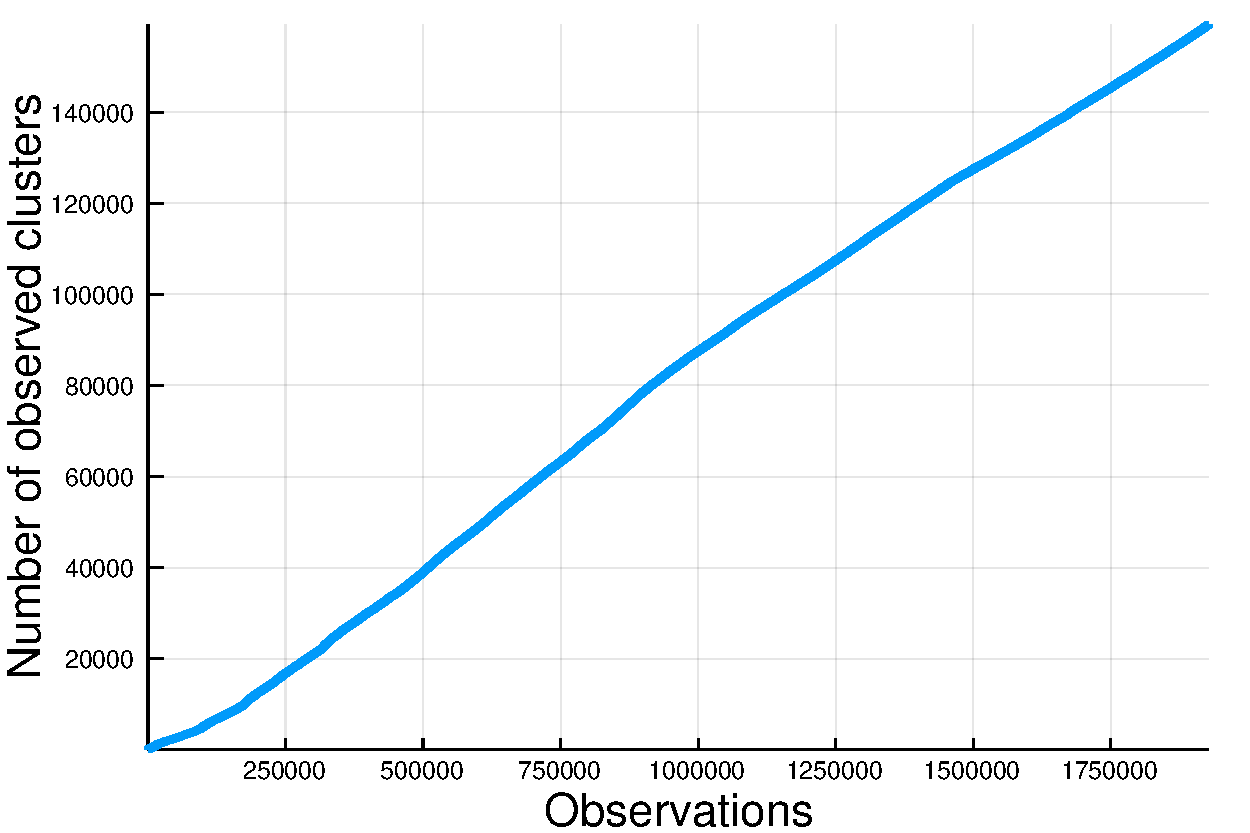
\includegraphics[width=0.485\textwidth]{fig/arrival_times_askubuntu.pdf}
  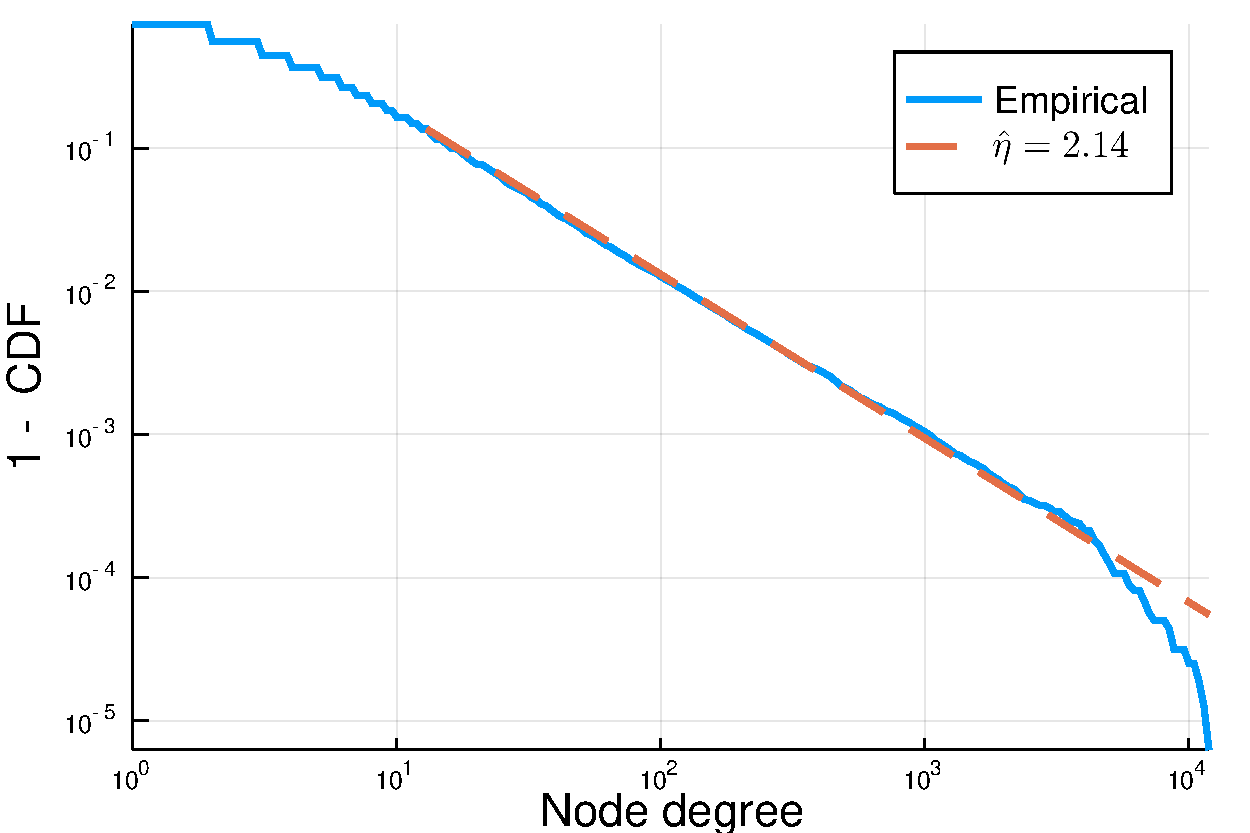
\includegraphics[width=0.485\textwidth]{fig/nodes_degre_power_law_askubuntu.pdf}
  \caption{Ask Ubuntu arrival process (left) and node degree distribution (right)}
  \label{fig:ppd}
\end{center}
\end{figure}


\vspace{\shrinkend}
\end{block}

\vspace{\shrink}


%----------------------------------------------------------------------------------------
%	Previous models
%----------------------------------------------------------------------------------------

\begin{block}{Models}
\textbf{Edge exchangeable} models \cite{CraneDempsey2017} \cite{cai2016} include \textbf{Exchangeable Gibbs partitions} and \textbf{Pitman--Yor process} (PYP).
\vspace{0.5\baselineskip}

\textbf{Preferential attachment} (PA) models include \textbf{Yule--Simon} (YS) model.
\vspace{0.5\baselineskip}

A \textbf{Beta Neutral-to-the-left model} (BNTL) \cite{Bloem2017} %for a sequence $\bfee\in\bbN^{\infty}$ 
is parameterized by $\alpha\in(-\infty,1)$ and arrival distribution $\aDist_\phi$ on $\bbN^{\infty}$. Distribution on $\mathbf{Z}$ is
\begin{align} 
  (T_1, T_2, ...) &\sim \Lambda_\phi \\
  \ee_{n+1} | \bfee_{n}, \bfT &= \begin{cases}\begin{aligned}
  	K_{n+1} & \text{ w.p. } 1 && \text{if } n+1 = T_{K_{n+1}} \\
  	j &\text{ w.p.} \propto (d_{j,n} - \alpha) && \text{otherwise} 
  	\end{aligned}\end{cases}
  \label{eq:bntl}
\end{align}

\vspace{16pt}

\begin{figure}[H]
\begin{center}
\begin{tikzpicture}[->,auto,node distance=3.6cm, thick,baseline=0,scale=1.3]

\tikzstyle{every node}=[scale=1.3]
                    
\def\pyp{(-0.9,-0.2) coordinate (a) circle (1.5cm)}
\def\ys{(-1,3.5) coordinate (b)  circle (1cm)}
\def\ex{(-3.5,-0.2) coordinate (c) ellipse (5.5cm and 2cm)}
\def\pa{(-2.4,3.5) coordinate (d) ellipse (3cm and 1.5cm)}
\def\bntl{(0.5,1.4) coordinate (e) ellipse (3.5cm and 4.2cm)}

\draw \pyp  node {PYP};
\draw \ys node {YS};
\draw \ex;
\draw node at (-5.5,-0.2) {Edge exch.};
\draw \pa;
\draw node at (-3.7, 3.5) {PA};
\draw \bntl;
\draw node at (2,2.2) {BNTL};
\end{tikzpicture}
\end{center}
\end{figure}


\textbf{Network properties}

\begin{table}
\begin{tabular}{l|l|l}
	& \textbf{Growth rate} & \textbf{Degree exponent, $\eta$} \\
	\hline
	Ask Ubuntu & Linear. & $\hat{\eta} = 2.14$ \\
	All SNAP datasets & Linear and sublinear. & $\hat{\eta} \in (1.5, 3)$ \\
	\hline
	Edge exchangeable models & Sublinear. $K_n = o(n)$ & $\eta \in (1,2)$ \\
    Yule--Simon model & Linear. $\Delta_j \simiid \text{Geom}(\beta)$ & $\eta \in (2,\infty)$ \\
    \textbf{BNTL models} & $\mathbf{T}$ \textbf{has law} $\Lambda_\phi$ & ${\eta \in (1,\infty)}$ \\
    
\end{tabular}
\end{table}


\vspace{\shrinkend}
\end{block}

\vspace{\shrink}


	
\end{column} % End of the first column

\begin{column}{.02\textwidth}\end{column} % Empty spacer column

\begin{column}{.47\textwidth} % The second column

%----------------------------------------------------------------------------------------
%	Inferece
%----------------------------------------------------------------------------------------

\vspace{\shrink}

\begin{block}{Inference \cite{bloem2018}}
BNTL models have \textbf{tractable inference} due to the factorisations
\begin{align} \label{eq:likelihoodfactorization}
\bbP_{\alpha,\phi}(\bfee_n) &= \bbP_{\alpha}(\bfee_n|\bfT_{K_n})\aDist_{\phi}(\bfT_{K_n}) \;, \\
 \label{eq:cppf}
  \bbP_\alpha[G(\bfee_n)|\bfT_{K_n}] &=   \frac{\Gamma(d_{1,n}-\alpha)}{\Gamma(n - K_n\alpha)} \prod_{j=2}^{K_n} \frac{\Gamma(T_j - j\alpha) \Gamma(d_{j,n} - \alpha)}{\Gamma(T_j - 1 - (j-1)\alpha)\Gamma(1-\alpha)} \;,
\end{align}
in particular the degree sequence $\bfd_n:=(d_{1,n},\dotsc,d_{{K_n},n})$ is a sufficient statistic for $\alpha$ conditional on $\mathbf{T}_{K_n}$.
\vspace{16pt}
\begin{center}
\begin{tabular}{lll}
	\textbf{Observation} & \textbf{Unobserved variables} \\
    \midrule
    End of edge sequence $\mathbf{Z}_n$ & $\alpha, \phi, \mathbf{\Psi}_{K_n}$ \\
    Vertex arrival-ordered graph & $\alpha, \phi, \mathbf{\Psi}_{K_n}, \mathbf{T}_{K_n}$ \\
    Unlabeled graph & $\alpha, \phi, \mathbf{\Psi}_{K_n}, \mathbf{T}_{K_n}$, $\sigma [K_n]$
\end{tabular}
\end{center}
\vspace{16pt}
\begin{center}
\begin{tabular}{l|l}
	\textbf{Variable} & \textbf{Gibbs sampling scheme} \\
    \midrule
    $\alpha$ & Slice sampling \\
    $\phi$ & Depends on family $\Lambda_\phi$ \\
    & \quad Conjugate updates possible e.g. $\Delta_j \sim \text{Geom}(\beta)$ \\
    $\mathbf{\Psi}_{K_n}$ & $\Psi_j | \bfee_n, \mathbf{\Psi}_{\setminus j} \sim \text{Beta}(d_{n,j} - \alpha, \bar{d}_{n,j-1} - (j-1)\alpha)$ \\
    & \quad where $\bar{d}_{n,j} = \sum_{i=1}^j d_{j,n}$, marginalise if $\mathbf{Z}_n$ not observed \\
    $\mathbf{T}_{K_n}$ & Assume Markov structure \\
    & \quad Simple update for $T_j$ -- can't move past neighbours \\
    $\sigma[K_n]$ & Swap proposal probability is cheap
\end{tabular}
\end{center}
\vspace{8pt}

For massive graphs with $\mathbf{Z}_n$ observed, \textbf{maximum a posterior} (or \textbf{maximum likelihood}) estimates for $\alpha, \phi$ computable from \eqref{eq:likelihoodfactorization}.




\vspace{\shrinkend}
\end{block}

\vspace{\shrink}


\begin{block}{Experiments}
\textbf{Gibbs sampler accuracy on synthetic data (500 edges)}
	\begin{table}[h]
%  \caption{Results of Gibbs sampling experiments on synthetic data $(\alpha^* = 0.75)$. The top four rows show results from each of four different BNTL models fit to a synthetic graph with 500 edges generated by the coupled $\PYP$ BNTL model; the bottom four rows show the same BNTL models fit to a synthetic graph with $\Geom(0.25)$-distributed interarrivals.}
  \label{tab:ess}
  \vspace*{-0.75\baselineskip}
  \begin{center}
  \resizebox{1.0\textwidth}{!}{
    \begin{tabular}{lllll}
    	Gen. arrival distn. & Inference model & $|\hat{\alpha} - \alpha^*|$ & $|\mathbf{\hat{S}} - \mathbf{S^*}|$ & Pred. log-lik.  \\
    	\hline
		$\PYP(1.0,0.75)$ &  $(\tau,\PYP(\theta,\tau))$ &  \textbf{0.046 $\pm$ 0.002}  &  \textbf{28.5 $\pm$ 0.7}  & -\textbf{2637.0 $\pm$ 0.1}  \\ 
		 
		$\PYP(1.0,0.75)$  &  $(\alpha,\Geom(\beta))$  &  {0.049 $\pm$ 0.004}  &  66.8 $\pm$ 1.2  & -2660.5 $\pm$ 0.7  \\ 
		\hline
		 
		$\Geom(0.25)$ & $(\tau,\PYP(\theta,\tau))$ &  0.086 $\pm$ 0.002  &  56.6 $\pm$ 1.3  & -2386.8 $\pm$ 0.1  \\  
		 
		$\Geom(0.25)$ & $(\alpha,\Geom(\beta))$ &  \textbf{0.043 $\pm$ 0.003}  &  \textbf{24.8 $\pm$ 0.8}  & -\textbf{2382.6 $\pm$ 0.2}  \\ 

    \end{tabular}
  }
  \end{center}
\end{table}

where $\mathbf{S} := \frac{1}{K_n - 1} \sum_{j>1} (\bar{d}_{j-1} - T_j)$ \\
\vspace{0.2\baselineskip}
\textbf{Scalability of Gibbs sampler ($\Geom(0.25)$ arrivals)}

\begin{table}[t]
  \label{tab:ess:scale:n}
  \vspace*{-0.25\baselineskip}
  \begin{center}
%  \resizebox{0.6\textwidth}{!}{
  	\begin{tabular}{l  ll}
  		 & $n=200$ &  $n=20000$ \\ 
 		\hline
		$|\hat{\alpha} - \alpha^*|$ & 0.12 $\pm$ 0.01 &  0.01 $\pm$ 0.00 \\ 
		 
		$|\hat{\beta} - \beta^*|$ &  0.02 $\pm$ 0.00  &    0.00 $\pm$ 0.00  \\ 
		 
		ESS &  0.90 $\pm$ 0.04  &   0.75 $\pm$ 0.08  \\  

		Runtime (s) &  21 $\pm$ 0   &  2267 $\pm$ 2  \\ 

  	\end{tabular}
  %}
  \end{center}
\end{table}

	 \textbf{Maximum likelihood parameter estimation for Ask Ubuntu}
	
	\begin{table}[!ht]
%\caption{MLEs on full datasets, and predictive log-likelihood for final 20\% of edges based on MLEs fit to the first 80\%, for three different BNTL models. Note that the uncoupled $\PYP(\theta,\tau)$ and $\Geom(\geom)$ interarrival models have the same $\hat{\alpha}$ due to the factorization in \eqref{eq:likelihoodfactorization}.}
\label{tab:mle_diagnostics}
\vspace*{-0.75\baselineskip}
\begin{center}
\resizebox{1.0\textwidth}{!}{
\begin{tabular}{lll | lllllll}
\multicolumn{3}{c}{Coupled $\PYP(\theta,\alpha)$}  & &  \multicolumn{2}{c}{Uncoupled $\PYP(\theta,\tau)$} &  & \multicolumn{3}{c}{$\Geom(\geom)$}                             \\
\cline{1-3} \cline{5-6} \cline{8-10}
$(\hat{\theta},\hat{\alpha})$ & $\hat{\eta}$           & Pred. l-l.            & $\hat{\alpha}$    & $(\hat{\theta},\hat{\tau})$ & Pred. l-l.     &     & $\hat{\beta}$  & $\hat{\eta}$   & Pred. l-l.                             \\
\hline
 (18080, 0.25) & 1.25   & -3.707e6              & -2.54            & (-0.99, 0.99)    & -3.678e6  &   &  0.083 & 2.32    & \textbf{-3.678e6}                                          
\end{tabular}
}
\end{center}
\end{table}


\vspace{\shrinkend}
\end{block}


\vspace{\shrink}

\begin{block}{Future work}

\begin{itemize}
	\item Scale MCMC inference to larger networks
	\item Variational inference
\end{itemize}
\vspace{\shrinkend}
\end{block}

\vspace{\shrink}

	
\begin{block}{Acknowledgements}
\footnotesize{
YWT, BBR, EM's research leading to these results has received funding from the
European Research Council under the European Union's Seventh Framework
Programme (FP7/2007-2013) ERC grant agreement no. 617071. EM and YWT gratefully acknowledge Microsoft Research and EPSRC for
partially funding EM's studentship. AF gratefully acknowledges funding from EPSRC grant no. EP/N509711/1.
}
	
\vspace{\shrinkend}
\end{block}

	
\vspace{\shrink}	
	
\begin{block}{References}
		
	%	\nocite{*} % Insert publications even if they are not cited in the poster
		\footnotesize{\bibliographystyle{unsrt}
			\bibliography{refs}}
\vspace{\shrinkend}		
\end{block}


%----------------------------------------------------------------------------------------

\end{column} % End of the second column

\begin{column}{.02\textwidth}\end{column} % Empty spacer column

\end{columns} % End of all the columns in the poster

\end{frame} % End of the enclosing frame

\end{document}
